%
%  untitled
%
%  Created by Johan Boissard [] on 2010-06-24.
%  Copyright (c) Johan Boissard. All rights reserved.
% hhh

\documentclass[a4paper,titlepage] {scrartcl}
\usepackage[T1]{fontenc}
\usepackage[utf8]{inputenc}
\usepackage{graphicx}
\usepackage{engord}
%\usepackage[english]{babel}
\usepackage{fancyhdr}
\usepackage{amsmath, amssymb}
\usepackage{comment}

\usepackage{listings}

%allows inclusion of url (hyperref is better than url) 
%ref: http://www.fauskes.net/nb/latextips/
\usepackage{hyperref}

%package for chemistry ie: \ce{(NH4)2SO4 -> NH4+ + 2SO4^2-} 
%ref:www.ctan.org/tex-archive/macros/latex/contrib/mhchem/mhchem.pdf
\usepackage[version=3]{mhchem}
%celsius + degrees
\usepackage{gensymb}
%to get last page
\usepackage{lastpage} % \pageref{LastPage}

%make use of the fullpage (no HUGE margins)
\usepackage{fullpage}
\usepackage{subfig}

%allows separating cell in table by diagonal line
\usepackage{slashbox}




%\renewcommand{\chaptername}{Laboratory}
%\setcounter{chapter}{5}

\usepackage{color}
\usepackage[usenames,dvipsnames, table]{xcolor}
% Include this somewhere in your document



\usepackage[absolute]{textpos}

%column  of multi row in tables
\usepackage{multirow}

%to have vertical text in table
\usepackage{rotating}


%%%%%%% a virer ici!!!!
\begin{comment}
%Fonts and Tweaks for XeLaTeX
\usepackage{fontspec,xltxtra,xunicode}
%\defaultfontfeatures{Mapping=tex-text}
%\setromanfont[Mapping=tex-text]{Hoefler Text}
\setsansfont[Scale=MatchLowercase,Mapping=tex-text]{Gill Sans}

\definecolor{shade}{HTML}{D4D7FE}	%light blue shade
\definecolor{text1}{HTML}{272727}		%text is almost black
\definecolor{headings}{HTML}{173849} 	%dark blue %%%dark red 70111
\definecolor{title}{HTML}{173849} 	%dark blue %%%dark red 70111

\usepackage{titlesec}				%custom \section
\end{comment}







\author{Johan Boissard}
\date{\today}
\title{Micro- \& Macro- Economics}
\begin {document}

%\maketitle
%\tableofcontents

\section{Loi Normale/Gauss/Cloche}

\paragraph{Propriété 1} % (fold)
\label{par:propriété_1}
\begin{equation}
	\mathbb P(X\geq x) = 1 -\mathbb P(X\leq x)
\end{equation}

% paragraph propriété_1 (end)

\paragraph{Propriété 2} % (fold)
\label{par:propriété_2}
Si $Z\sim \mathcal N(0,1)$

\begin{equation}
	\mathbb P(Z\leq z) = \Phi(z)
\end{equation}
% paragraph propriété_2 (end)

\paragraph{Propriété 3} % (fold)
\label{par:propriété_3}
Si $X\sim \mathcal N(\mu, \sigma^2)$ et $Z\sim \mathcal N(0, 1)$, on fait le \textbf{changement de variable} suivant
\begin{equation}
	Z = \frac{X-\mu}{\sigma}
\end{equation}
qui implique

\begin{equation}
	z = \frac{x-\mu}{\sigma}
\end{equation}

\begin{eqnarray}
	\mathbb P(X\leq x) &= \mathbb P(Z\leq z) &= \Phi\left(z\right)\nonumber\\
	 &= \mathbb P\left(Z\leq \frac{x-\mu}{\sigma}\right) &=\Phi\left(\frac{x-\mu}{\sigma}\right) 
\end{eqnarray}
% paragraph propriété_3 (end)

\paragraph{Propriété 4} % (fold)
\label{par:propriété_4}
Si $Z\sim\mathcal N(0,1)$

\begin{equation}
	\mathbb P(Z\leq -z) = 1-\mathbb P(Z\geq z) = 1 -\Phi(z)
\end{equation}
% paragraph propriété_4 (end)

\paragraph{Propriété 5} % (fold)
\label{par:propriété_5}

$\Phi(z)$ est défini comme la fonction de répartition de la loi de densité de la loi normale ($Z\sim\mathcal N(0,1)$, représenté ici par $f_Z(z)=\phi(z)$), elle a les propriétés suivantes

\begin{eqnarray}
	\Phi(x) &=& \int_{-\infty}^x \phi(x)dx\\
	\Phi(-\infty) &=& 0\\ 
	\Phi(\infty) &=& 1\\
	\frac{d\Phi(z)}{dz}&>&0
\end{eqnarray}

% paragraph propriété_5 (end)

\paragraph{Propriété 6} % (fold)
\label{par:propriété_6}
\begin{itemize}
	\item $68\%$ des valeurs sont dans $\mu\pm \sigma$
	\item $95.54\%$ des valeurs sont dans $\mu\pm 2\sigma$
\end{itemize}
% paragraph propriété_6 (end)

\paragraph{Propriété 7} % (fold)
\label{par:propriété_7}
\begin{itemize}
	\item $\Phi(0) = 50\%$
	\item $\Phi(1.69) = 95\%$
	\item $\Phi(1.96)=97.5\%$
\end{itemize}
% paragraph propriété_7 (end)


\begin{figure}[!htbp]
	\centering
		\includegraphics[height=3.5in]{img.png}
	\caption{Illustration de la courbe de Gauss}
	\label{fig:img}
\end{figure}

\begin{figure}[htbp]
	\centering
		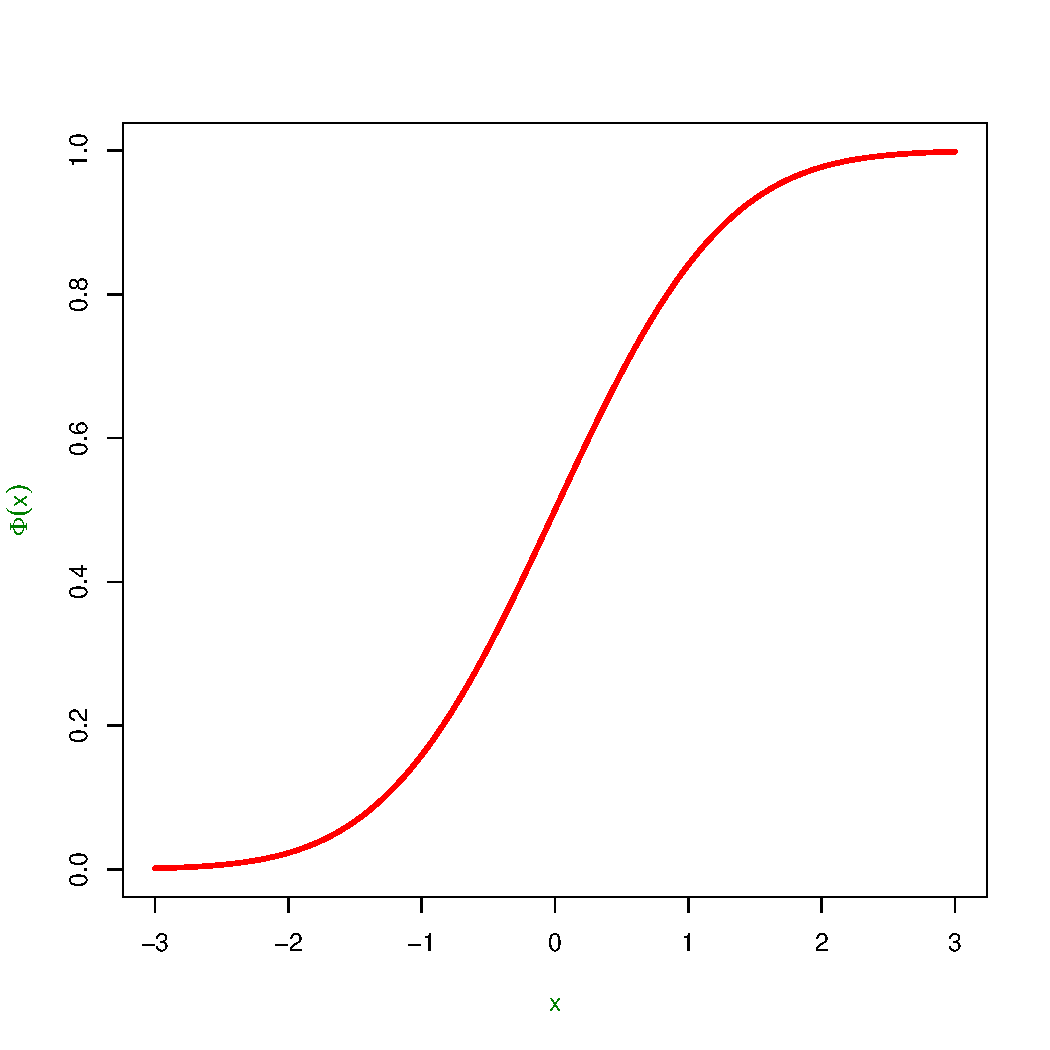
\includegraphics[height=4.5in]{cumnorm.pdf}
	\caption{Illustration de la fonction de répartition de la distribution normale}
	\label{fig:cumnorm}
\end{figure}


\end{document}
